\documentclass[11pt]{article}
\usepackage[margin=1in]{geometry}
\usepackage[T1]{fontenc}
\usepackage[utf8]{inputenc}
\usepackage{lmodern}
\usepackage{graphicx}
\usepackage{booktabs}
\usepackage{array}
\usepackage{hyperref}
\usepackage{caption}
\usepackage{subcaption}
\usepackage{xcolor}

\hypersetup{
  colorlinks=true,
  linkcolor=blue!50!black,
  citecolor=blue!50!black,
  urlcolor=blue!50!black
}

\title{Trinity Storyworld Reasoning Benchmark\\A Bioethics Trace Case Study}
\author{GPTStoryworld Benchmark Package}
\date{}

\begin{document}
\maketitle

\begin{abstract}
We present a compact Trinity-only benchmark for comparing reasoning style in storyworld play traces. The benchmark is derived from Trinity Thinking runs on a bioethics escalation storyworld and scores each pick-time reasoning trace on five heuristic dimensions: stakeholder breadth, tradeoff depth, reversibility, uncertainty, and legitimacy. We compare two prompt variants, v2 and v3, and find that v3 yields broader stakeholder framing, more explicit legitimacy language, and somewhat stronger tradeoff and uncertainty handling, while reversibility remains unchanged.
\end{abstract}

\section{Introduction}
Reasoning benchmarks often focus on answer accuracy or external judgments. That misses a different property that matters in moral and constitutional storyworlds: the shape of the model's own deliberation. This case study treats the model's pick-time reasoning text as the object of analysis and asks a narrower question: does the reasoning itself become broader, more explicit, and more institutionally aware when the storyworld prompt is sharpened?

The data here comes from Trinity Thinking playthroughs on two versions of the same bioethics world. Both versions use the same broad moral frame, but the v3 version makes the choice structure and the legitimacy stakes more explicit. Other model families and the secret-ending play environment are outside this release and are treated as follow-on slices.

\section{Related Work}
This benchmark sits between three common evaluation styles:
\begin{itemize}
  \item outcome-oriented benchmarks that score the final answer or action
  \item judge-based evaluations that ask a separate model to grade a completion
  \item trace-oriented analyses that inspect the model's own reasoning text
\end{itemize}

The present case study follows the third path. It is closer to a reasoning-process audit than to a classical accuracy benchmark. That matters in storyworld settings because the output is not a single answer, but a sequence of constrained moral choices whose justification style is itself part of the object of study.

\section{Benchmark Design}
The benchmark scores each reasoning trace from 1 to 5 on five dimensions:
\begin{itemize}
  \item stakeholder breadth: how many affected parties or institutions are explicitly named
  \item tradeoff depth: whether the trace compares concrete harms and benefits
  \item reversibility: whether it addresses rollback, contingency, or irreversibility
  \item uncertainty: whether it distinguishes facts from guesses or hedges appropriately
  \item legitimacy: whether it invokes public trust, oversight, accountability, or public record
\end{itemize}

The scoring is heuristic and text-based. It is designed for comparative analysis of reasoning style, not for ground-truth moral grading.

\subsection{Rubric Rules}
The published scorer uses the pick-time reasoning text only. It does not consume the prompt body, the storyworld scene text, or the reaction payload. Each dimension is scored by phrase-trigger rules:
\begin{itemize}
  \item stakeholder breadth rises when the trace names more affected parties or institutions
  \item tradeoff depth rises when the trace compares alternatives or uses explicit tradeoff language
  \item reversibility rises when the trace mentions rollback, contingency, revisiting, or undoing
  \item uncertainty rises when the trace acknowledges unknowns, limits, or conditional reasoning
  \item legitimacy rises when the trace names public trust, oversight, accountability, or the public record
\end{itemize}

The intent is not to perfectly measure moral quality. The intent is to create a stable, inspectable proxy for reasoning breadth that can be reproduced across runs.

\section{Data}
We analyzed 69 Trinity play traces:
\begin{itemize}
  \item v2 run: 36 traces
  \item v3 run: 33 traces
\end{itemize}

Each row in the published benchmark contains:
\begin{itemize}
  \item the run label
  \item encounter and step identifiers
  \item the selected option id and text
  \item the extracted reasoning text
  \item per-dimension scores
  \item a short evidence payload showing which phrases triggered each dimension score
\end{itemize}

\section{Method}
The published benchmark is built from the model's pick-time reasoning text rather than the full story prompt. This matters because the prompts are intentionally rich and would otherwise inflate the scores with storyworld scaffolding. Using the reasoning text only makes the benchmark more reflective of the model's own deliberative style.

In implementation terms, the scorer lowercases the pick-time trace text, applies a small phrase-trigger rubric for each dimension, maps trigger counts to integer scores on a 1--5 scale, and averages the five dimensions into an overall score. That makes the export deterministic and easy to reproduce, while still surfacing differences in reasoning breadth and institutional awareness.

\section{Results}
The v3 run is stronger on every tracked dimension except reversibility, which stays flat.

\subsection{Aggregate Means}
\begin{itemize}
  \item v2 overall score: 1.428
  \item v3 overall score: 1.715
  \item delta: +0.287
\end{itemize}

\subsection{Dimension Deltas}
\begin{itemize}
  \item stakeholder breadth: +0.462
  \item tradeoff depth: +0.186
  \item reversibility: +0.000
  \item uncertainty: +0.245
  \item legitimacy: +0.543
\end{itemize}

\begin{table}[t]
\centering
\caption{Trinity bioethics reasoning benchmark results for v2 and v3.}
\label{tab:trinity_reasoning_results}
\begin{tabular}{lrrrrrrr}
\hline
Run & Rows & Overall & Stakeholder & Tradeoff & Reversibility & Uncertainty & Legitimacy \\
\hline
v2 & 36 & 1.428 & 2.417 & 1.056 & 1.000 & 1.028 & 1.639 \\
v3 & 33 & 1.715 & 2.879 & 1.242 & 1.000 & 1.273 & 2.182 \\
\hline
\end{tabular}
\vspace{0.6em}

\centering
\begin{tabular}{lr}
\hline
Metric & Delta \\
\hline
Overall & +0.287 \\
Stakeholder breadth & +0.462 \\
Tradeoff depth & +0.186 \\
Reversibility & +0.000 \\
Uncertainty & +0.245 \\
Legitimacy & +0.543 \\
\hline
\end{tabular}
\end{table}


\section{Interpretation}
Trinity Thinking appears to operate as a stable policy follower with coherent but narrow moral framing. The v3 prompt variant pushes the model to mention more stakeholders and more institutional stakes, and it slightly improves tradeoff and uncertainty language. The most visible shift is legitimacy: v3 more often refers to trust, oversight, accountability, or public record.

That said, Trinity does not suddenly become a deep pluralist deliberator. The reversibility dimension remains flat, and the model still favors conservative closure-oriented moves. The benchmark therefore measures a meaningful but bounded improvement in reasoning style rather than a wholesale change in moral strategy.

\section{Discussion}
This case study is useful for at least three reasons:
\begin{enumerate}
  \item It captures reasoning style directly from the model rather than from an external judge.
  \item It distinguishes prompt-driven structure from model-intrinsic deliberative breadth.
  \item It produces a compact, publishable artifact set with both quantitative summaries and qualitative trace examples.
\end{enumerate}

For the broader research agenda, the result suggests that storyworld design can function as a controllable lens on reasoning style. Small prompt changes can materially alter what the model says it is weighing, even when the chosen actions remain conservative.

\begin{figure}[htbp]
  \centering
  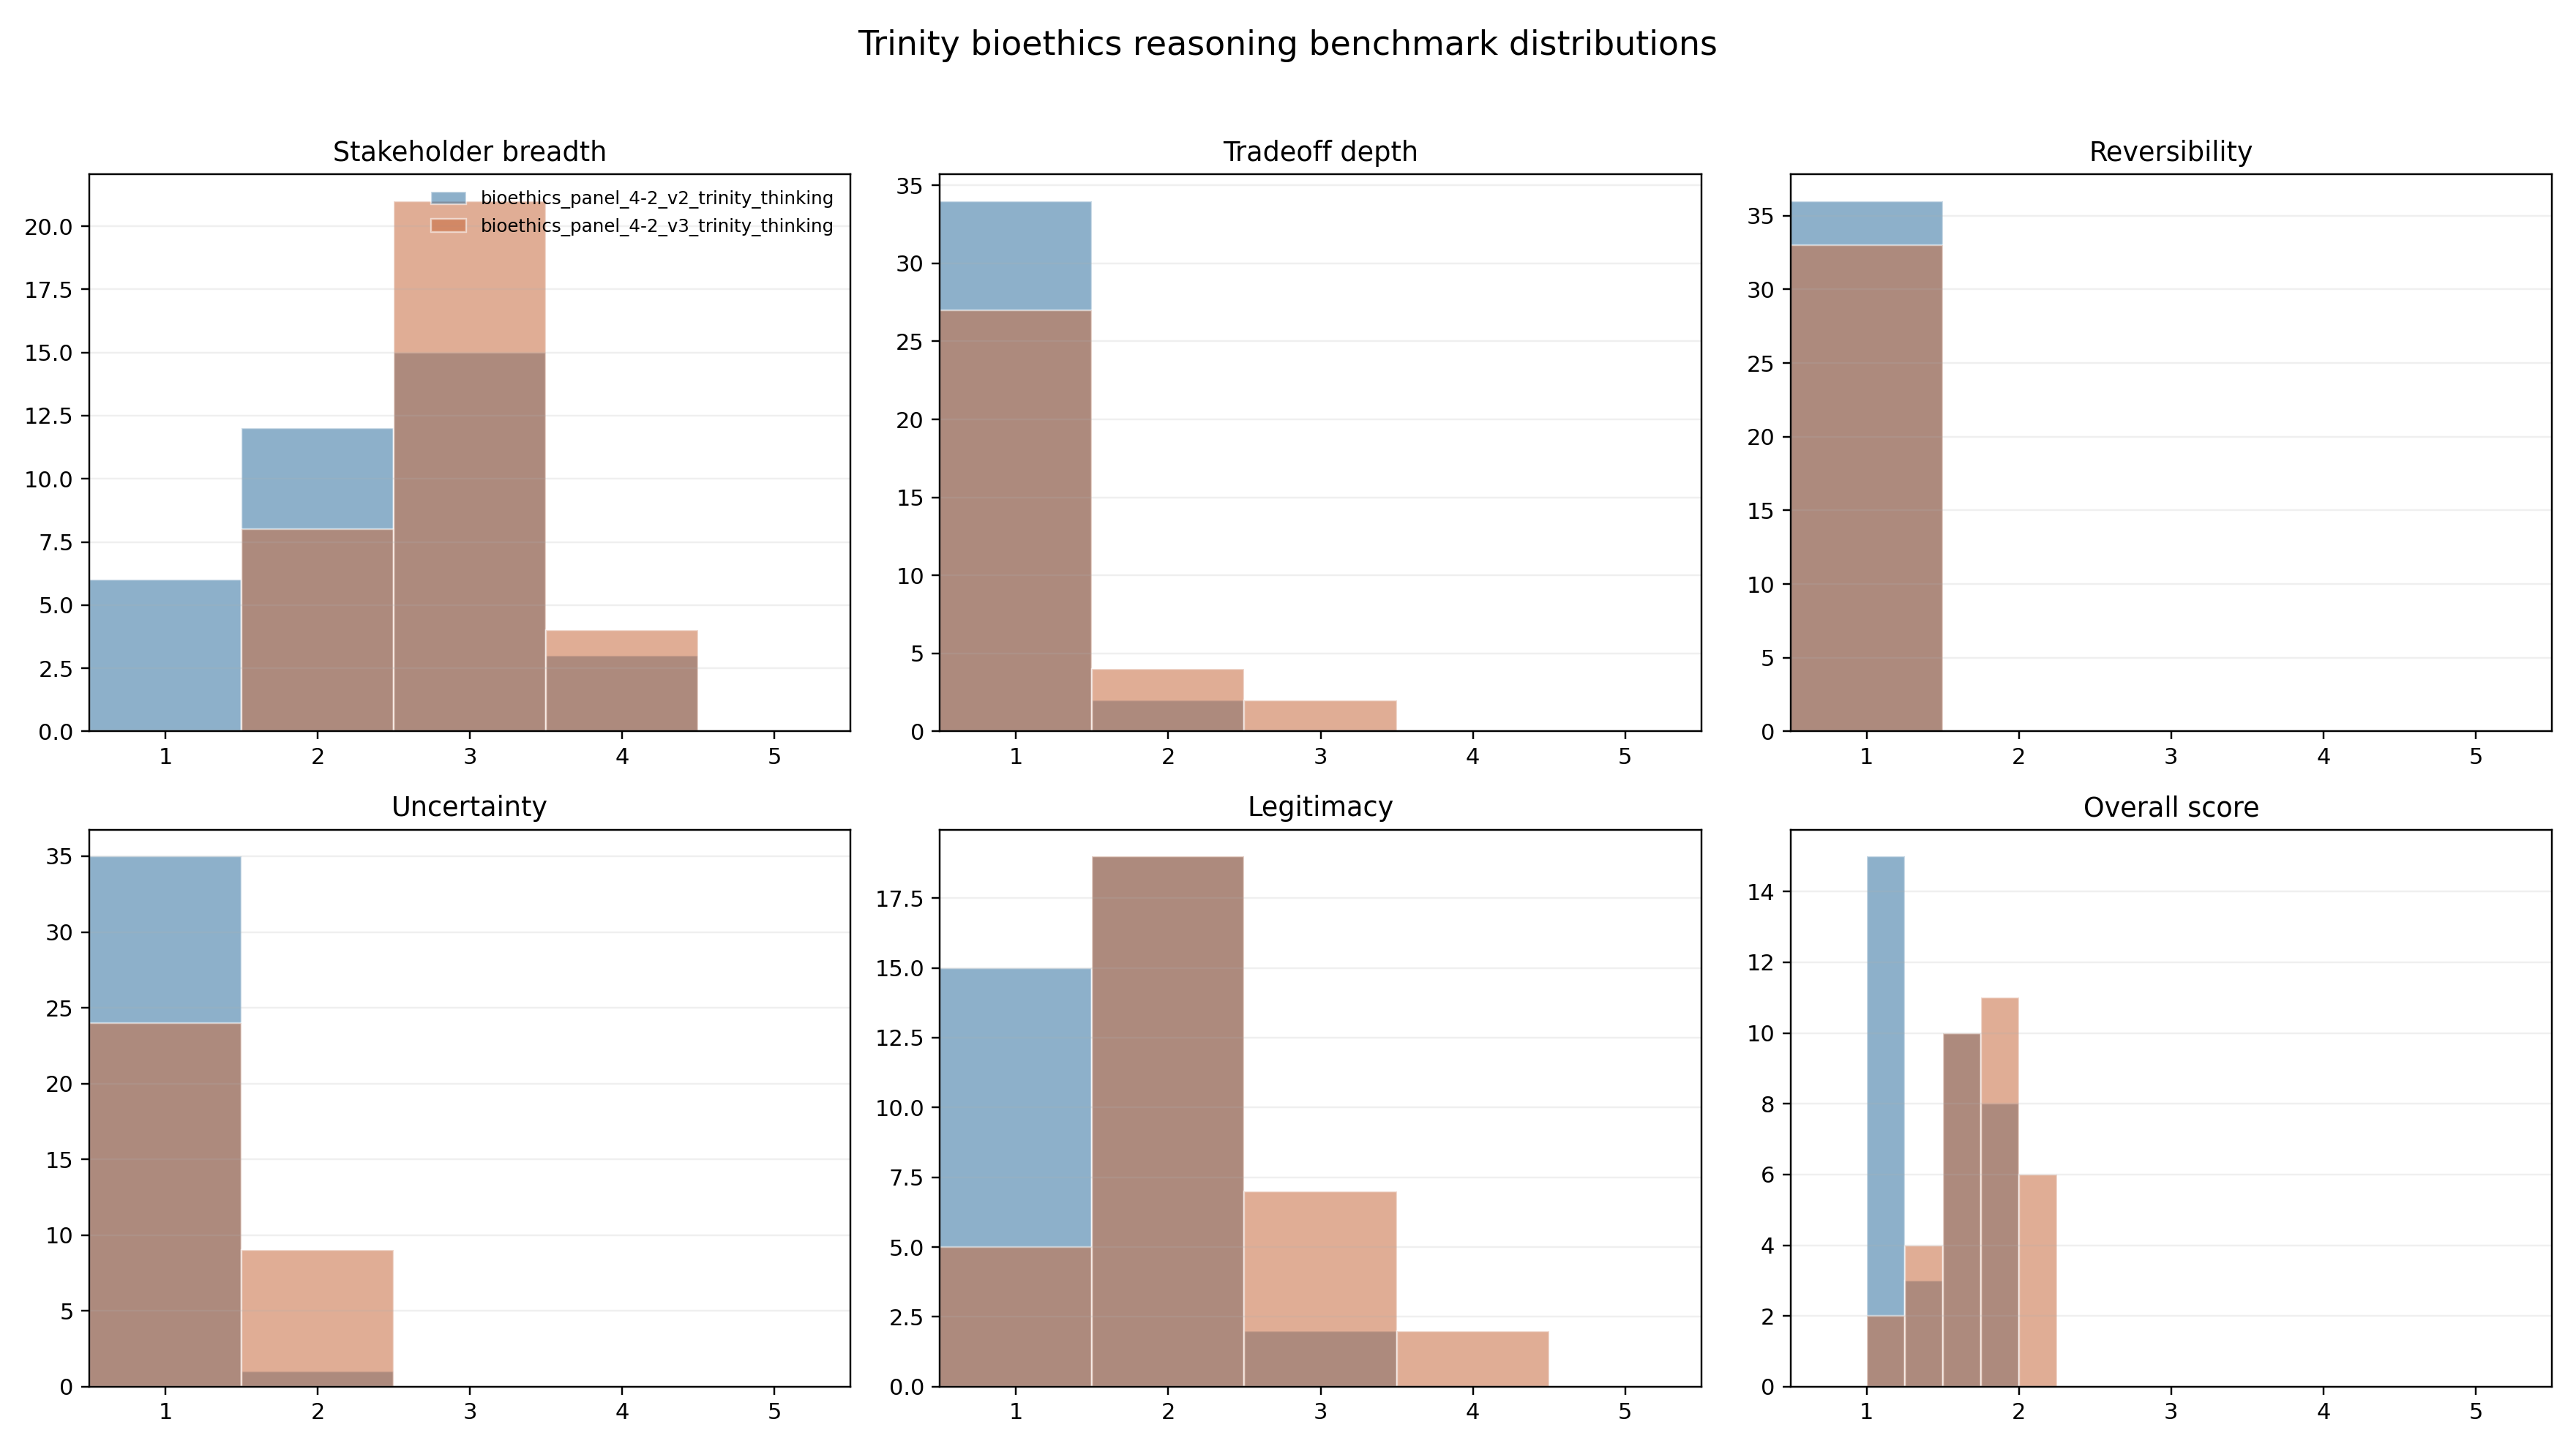
\includegraphics[width=0.95\linewidth]{figures/dimension_histograms.png}
  \caption{Overlaid histograms of the five rubric dimensions plus the overall score for v2 and v3.}
\end{figure}

\begin{figure}[htbp]
  \centering
  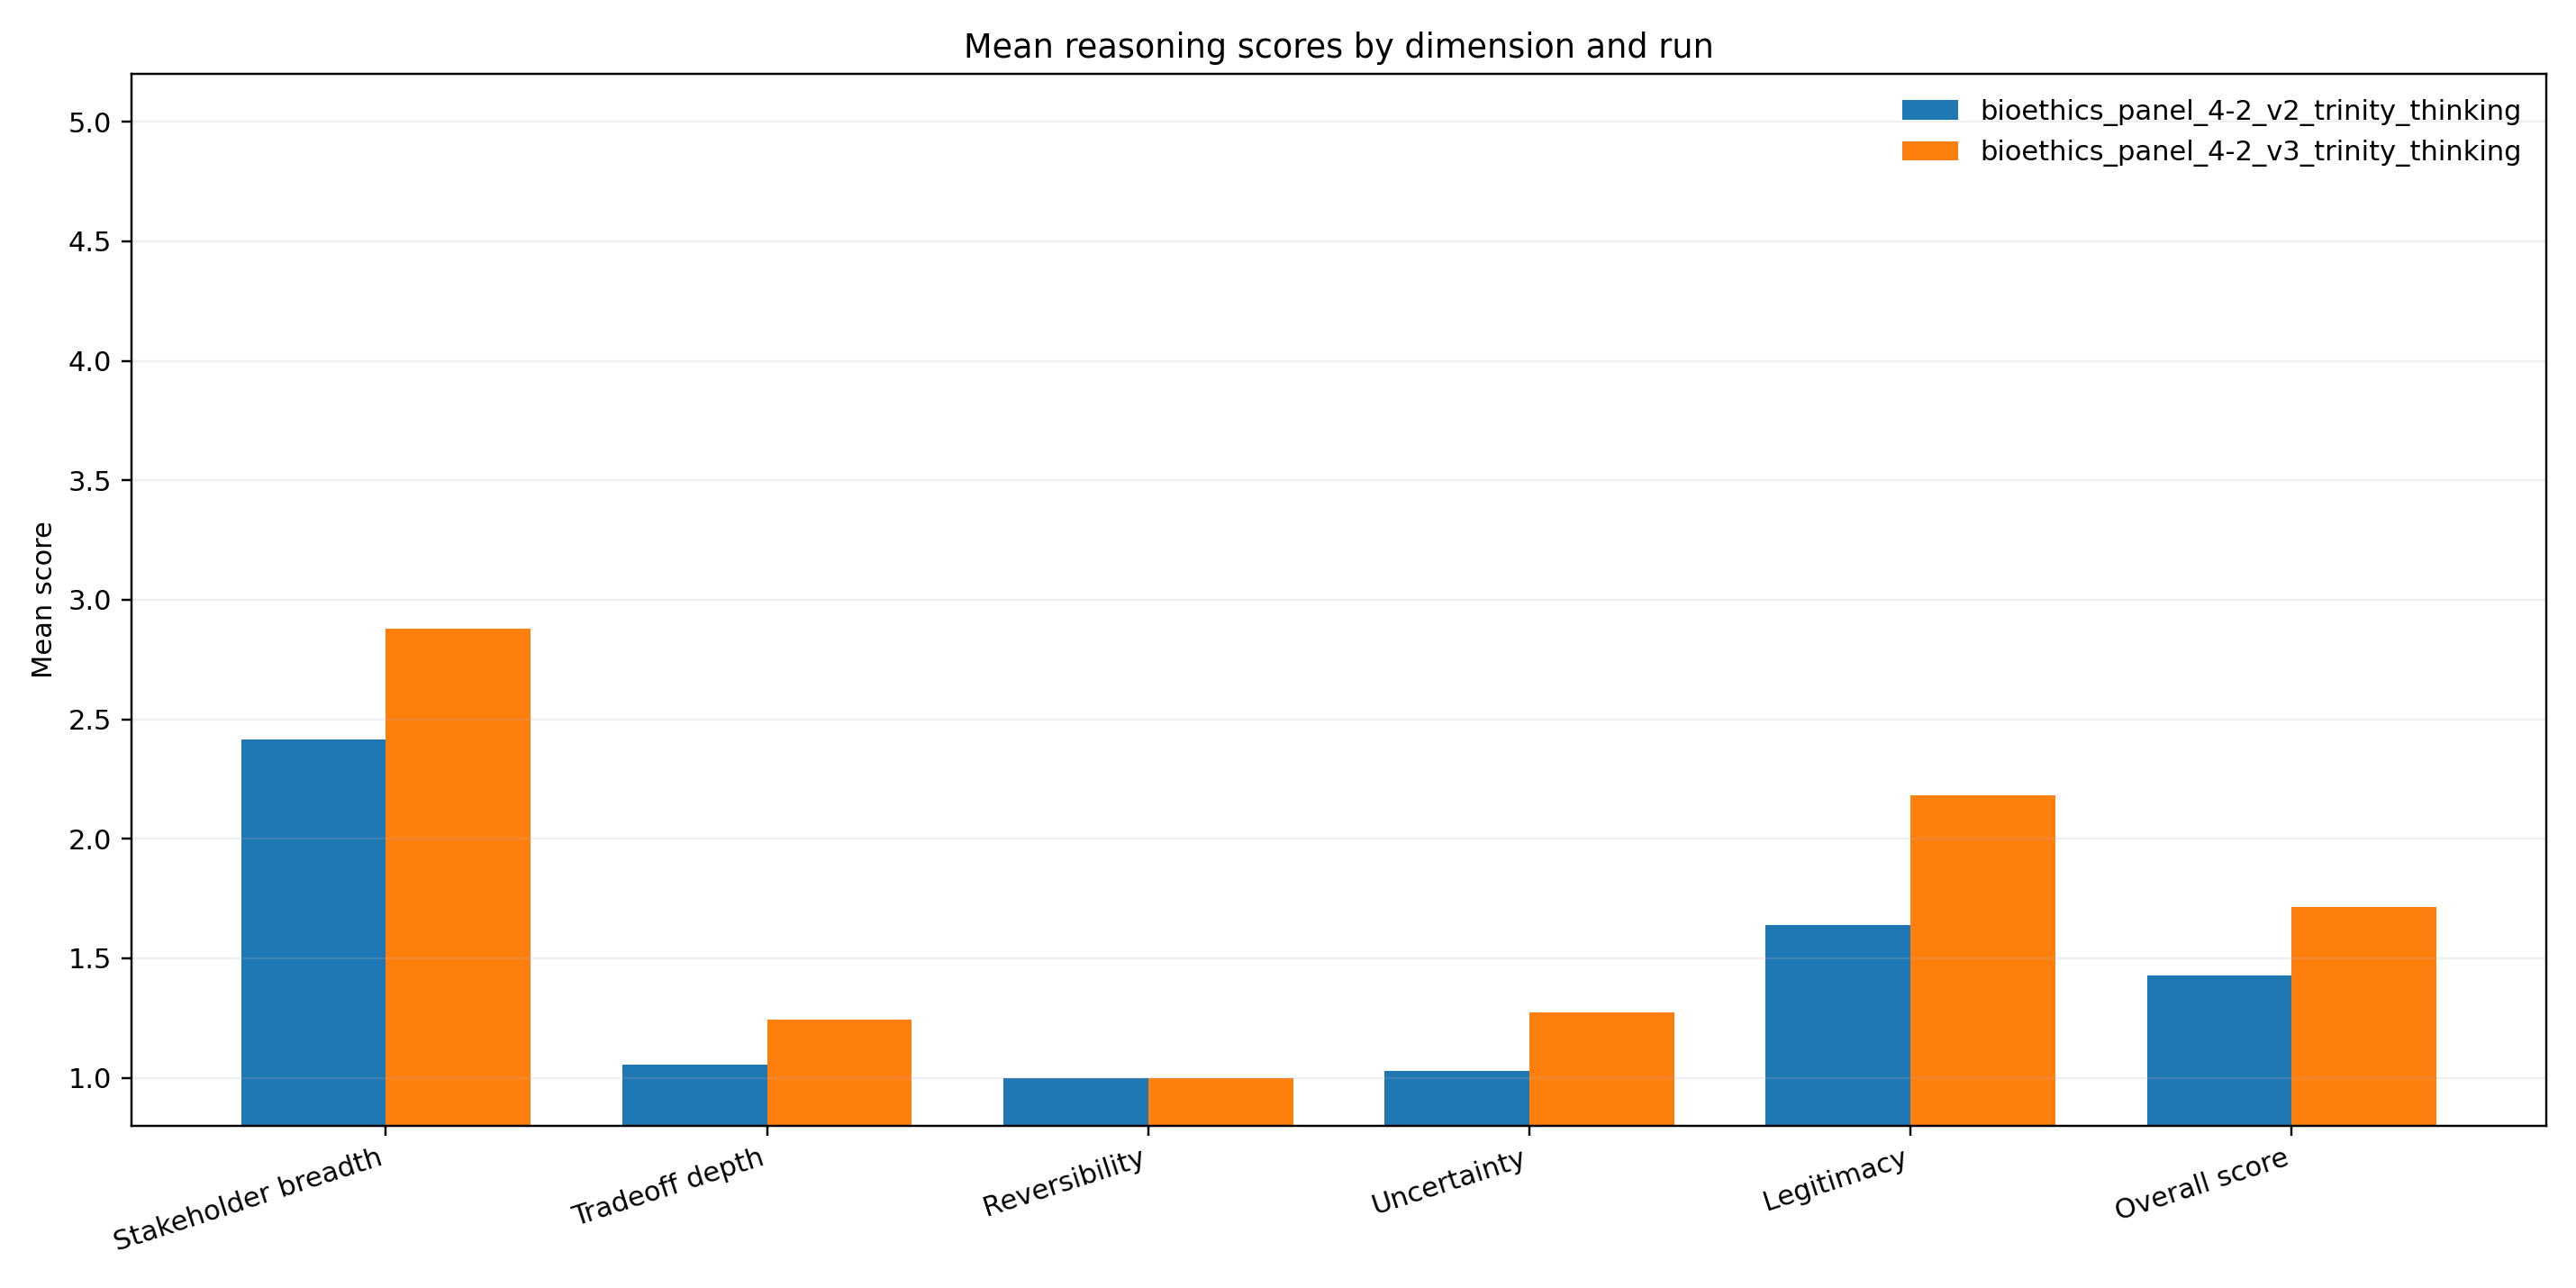
\includegraphics[width=0.95\linewidth]{figures/run_mean_bars.png}
  \caption{Side-by-side mean scores for each dimension, comparing v2 and v3.}
\end{figure}

\begin{figure}[htbp]
  \centering
  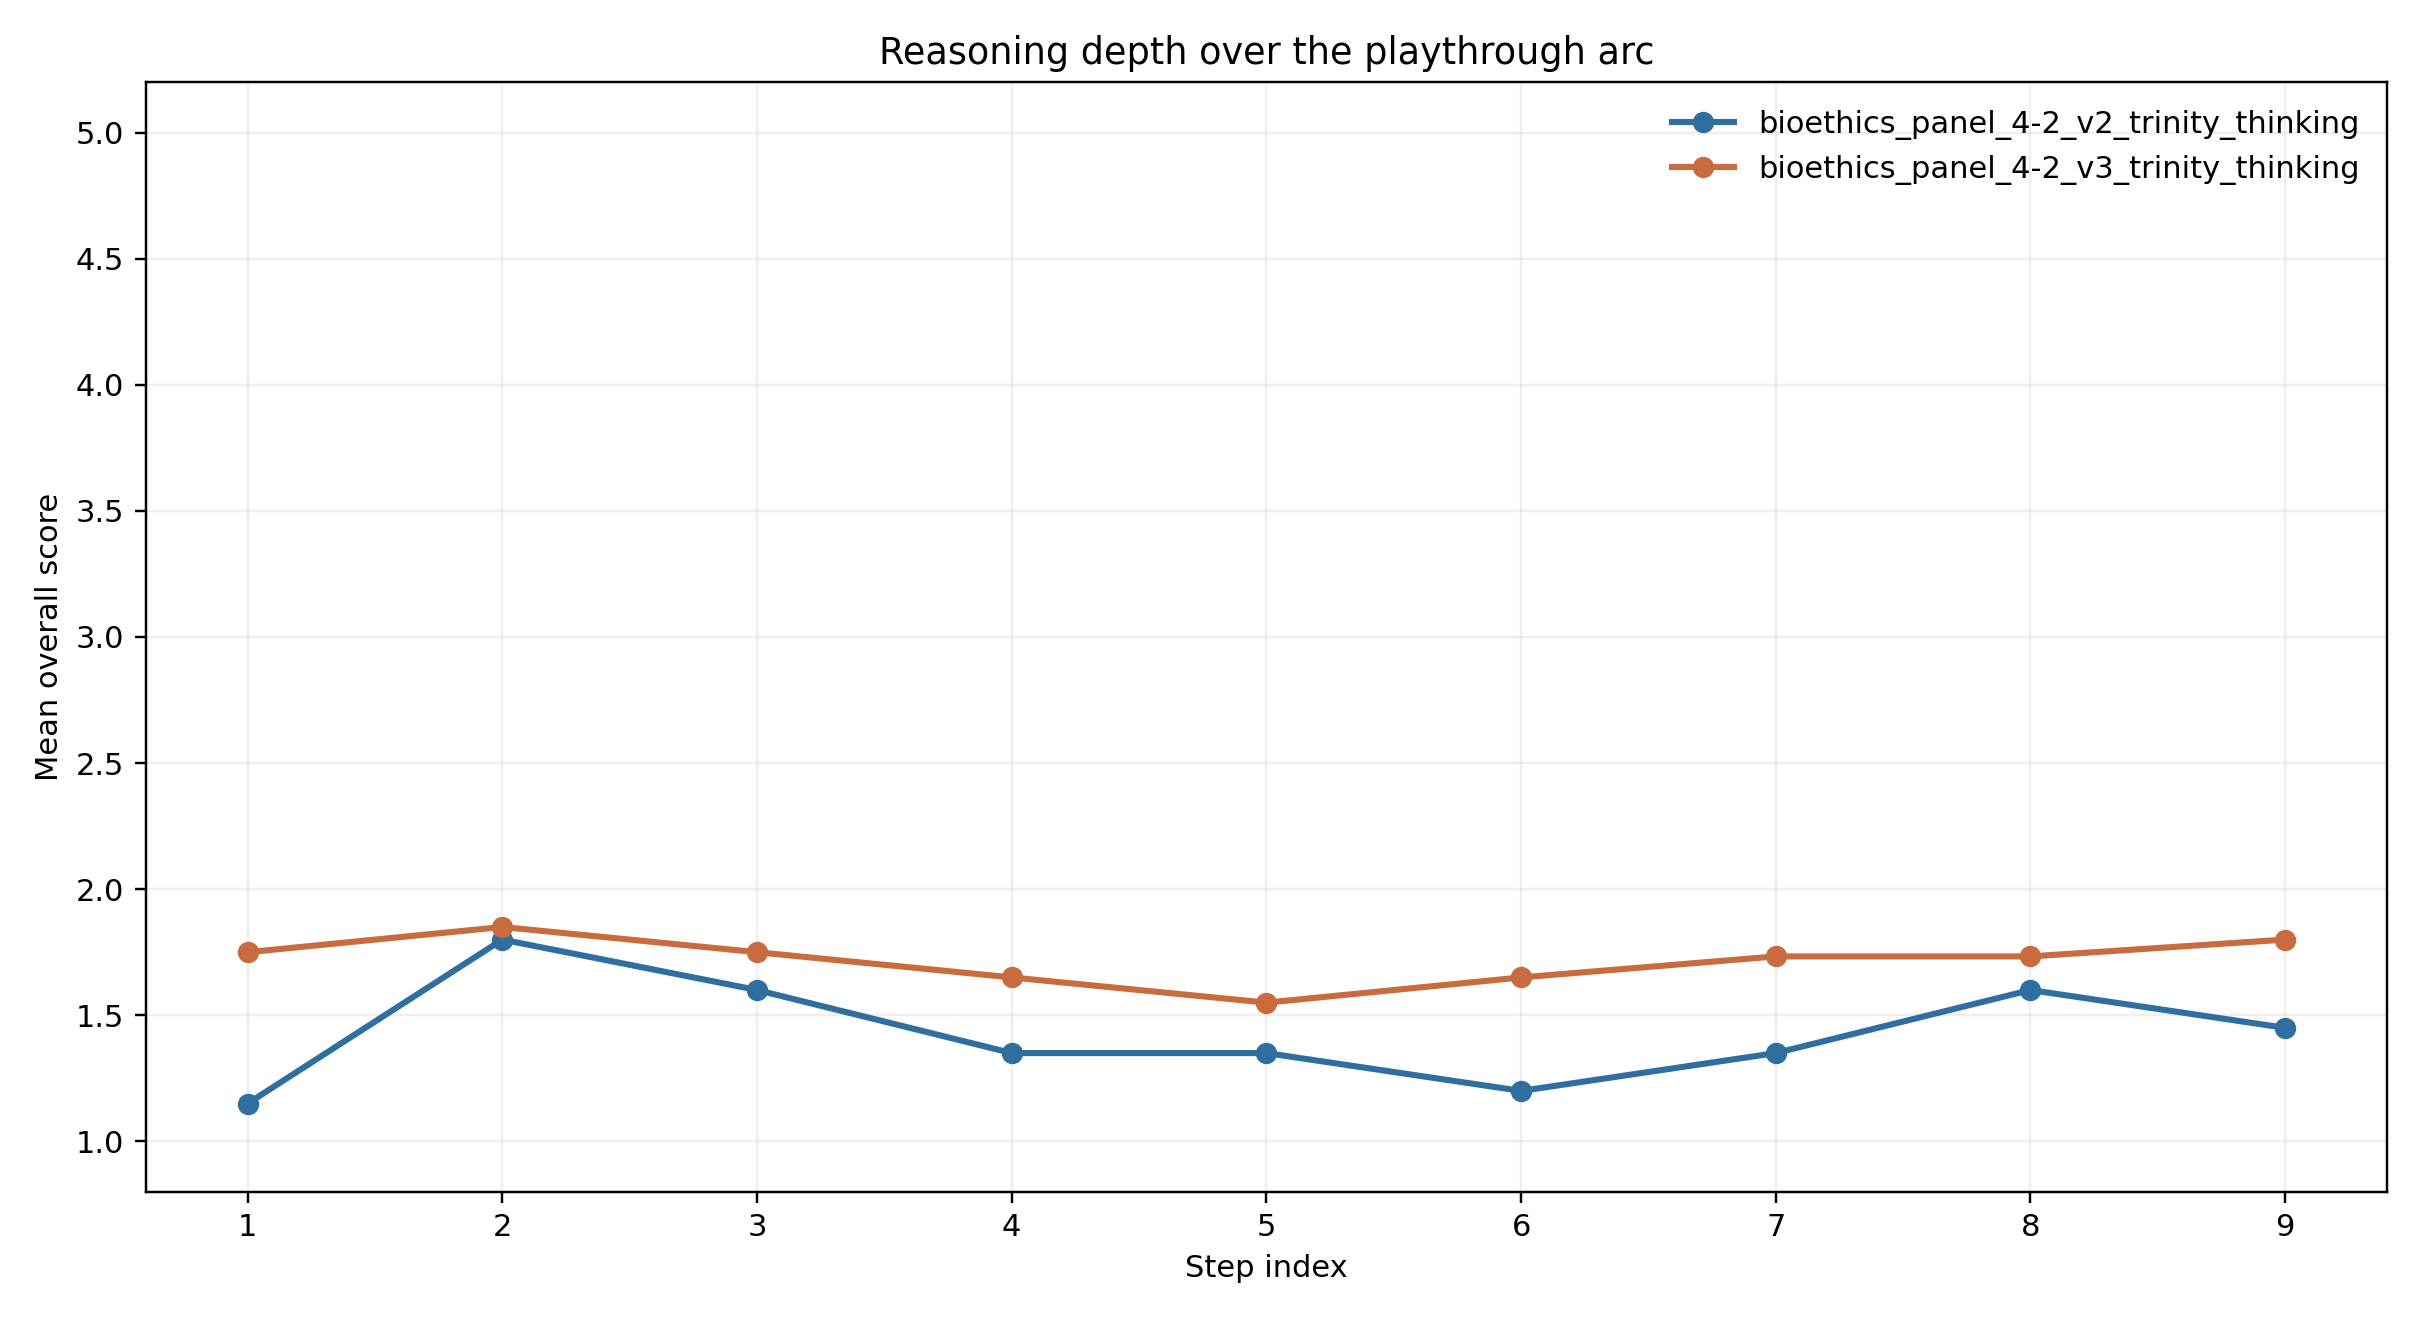
\includegraphics[width=0.9\linewidth]{figures/step_means.png}
  \caption{Mean overall reasoning score across the playthrough arc, showing how the two runs evolve over step index.}
\end{figure}

\section{Limitations}
This benchmark is intentionally heuristic.
\begin{itemize}
  \item It uses simple rubric-based scoring rather than human annotation or model-based judgment.
  \item It is sensitive to the wording of the storyworld prompts and to the trace format.
  \item It should not be interpreted as a ground-truth moral capability score.
  \item The current release covers only one model family and one storyworld family.
\end{itemize}

\section{Conclusion}
The Trinity bioethics case study shows that a storyworld benchmark can surface differences in reasoning style even when the model's final action policy remains conservative. V3 is the better reasoning trace set by this rubric, mainly because it expands stakeholder and legitimacy language without changing the underlying reversibility pattern. The next planned slices are the secret-ending play environment, an `o3-mini` contrast run, an Arcee model run, and a Codex webhook benchmark of a frontier model.

\end{document}
